\documentclass{article}


\usepackage{tikz}
\usetikzlibrary{%
    decorations.pathreplacing,%
    decorations.pathmorphing%
}
\begin{document}
\pagestyle{empty}

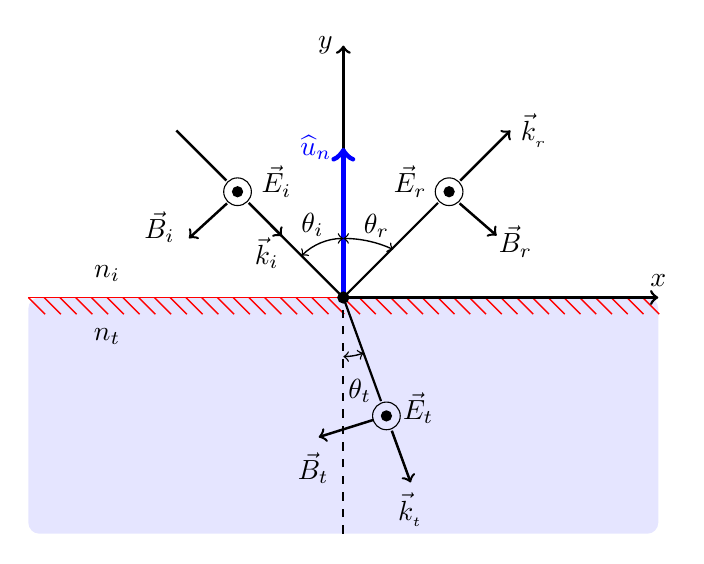
\begin{tikzpicture}[
    media/.style={font={\footnotesize\sffamily}},
    wave/.style={
        decorate,decoration={snake,post length=1.4mm,amplitude=2mm,
        segment length=2mm},thick},
    interface/.style={
        % The border decoration is a path replacing decorator. 
        % For the interface style we want to draw the original path.
        % The postaction option is therefore used to ensure that the
        % border decoration is drawn *after* the original path.
        postaction={draw,decorate,decoration={border,angle=-45,
                    amplitude=0.3cm,segment length=2mm}}},
    ]
    % Round rectangle
    \fill[blue!10,rounded corners] (-4,-3) rectangle (4,0);
    % Interface
    \draw[red,line width=.5pt,interface](-4,0)--(4,0);
    % Vertical dashed line
    \draw[dashed,black,line width=.8pt](0,-3)--(0,0);
    % Coordinates system
    \draw[<->,line width=1pt] (4,0) node[above]{$x$}-|(0,3.2) node[left]{$y$};
     %Unitary normal vector Un 
     \draw[->,blue,line width=2pt]
     (0:0cm)--(90:1.9cm)node[left]{$\widehat{u}_n$};
    % Incidence
    \draw[->,line width=.9pt](135:1.7cm)--(135:1.1cm);
     \path (0,0)++(141:0.9cm)node[left]{$\vec{k}_i$};
    \filldraw[fill=black,line width=1pt](135:1.9cm) circle(1.5pt); 
    \draw [black](135:1.9cm)circle (5pt); 
    \draw[black,line width=.8pt](0:0cm)--(135:1.3cm);
    \draw[->,line width=.9pt](141:1.9cm)--(159:2.1cm);
    \path (0,0)++(159:2.5cm)node{$\vec{B}_i$};
    \draw[-,line width=.9pt](135:2.1cm)--(135:3cm);
    \path (0,0)++(113:1cm)node{$\theta_i$};
    \draw[<->,black,line width=.5pt](0,0.75)arc(90:135:.75cm);
    \path (0,0)++(120:1.7cm)node{$\vec{E}_i$};
    % Transmission
    \draw[->,line width=.9pt](-70:1.8cm)
         --(-70:2.5cm)node[below]{$\vec{k}_{_{t}}$};
    \filldraw[fill=black,line width=1pt](-70:1.6cm) circle(1.5pt); 
    \draw [black](-70:1.6cm)circle (5pt);   
    \draw[black,line width=.8pt](0:0cm)--(-70:1.4cm);
    \draw[->,line width=.9pt](-76:1.6cm)--(-100:1.8cm);
    \path (0,0)++(-100:2.2cm)node{$\vec{B}_t$};
    \path (0,0)++(-80:1.2cm)node{$\theta_t$};
    \draw[<->,black,line width=.5pt] (0,-0.75) arc (-90:-70:.75cm);
    \path (0,0)++(-56:1.7cm)node{$\vec{E}_t$};
    % Reflection
    \draw[->,line width=.9pt]
         (45:2.1cm)--(45:3cm)node[right]{$\vec{k}_{_{r}}$};
    \filldraw[fill=black,line width=1pt](45:1.9cm) circle(1.5pt); 
    \draw [black](45:1.9cm)circle (5pt); 
    \path (0,0)++(65:1cm) node{$\theta_r$};
    \draw[black,line width=.8pt](0:0cm)--(45:1.7cm);
    \draw[->,line width=.9pt](39:1.9cm)--(22:2.1cm);
    \path (0,0)++(18:2.3cm)node{$\vec{B}_r$};
    \draw[<->,black,line width=.5pt] (0,0.75)arc(90:65:1.5cm);
     \path (0,0)++(60:1.7cm)node{$\vec{E}_r$};
    % Media names
    \path(0,0)++ (-3,.3)  node {$n_i$}
              (0,0)++ (-3,-.5) node[line width=.7pt] {$n_{t}$};
    \filldraw[black](0,0) circle(2pt);
    %\draw [black](0,0)circle (6pt);
    % $x$ axis
    %\filldraw[fill=white,line width=1pt](0,0)circle(.12cm);
    %\draw[line width=.6pt] (0,0)
                          %+(-135:.10cm) -- +(45:.10cm)
                          %+(-45:.1cm) -- +(135:.10cm);
    % Interface pointer
    %\draw[-latex,thick](3.2,0.5)node[right]{$\mathsf{S_{1,2}}$}
         %to[out=180,in=90] (3,0);
    % To-paths are really useful for drawing curved lines. The above
    % to path is equal to:
    %
    %\draw[-latex,thick](3.2,0.5)node[right]{$\mathsf{S_{1,2}}$}
        % ..controls +(180:.2cm) and +(up:0.25cm) .. (3,0);
    % Internally the to path is translated to a similar bezier curve,
    % but the to path syntax hides the complexity from the user. 

\end{tikzpicture}

\include{paralela}
\end{document}